% !Mode:: "TeX:UTF-8"
\documentclass[QA.tex]{subfiles}

\begin{document}
%-=-=-=-=-=-=-=-=-=-=-=-=-=-=-=-=-=-=-=-=-=-=-=-=
%
%	CHAPTER
%
%-=-=-=-=-=-=-=-=-=-=-=-=-=-=-=-=-=-=-=-=-=-=-=-=

%%================================================================
\chapter{20180108}\label{ch180108}
%----------------------------------------------------------------------------------------

\begin{qst}\label{Q2018010801}
谁有\LaTeX{}数学建模美赛模板呢?\index{建模模板}
\end{qst}
\ans 群主网站上\href{http://www.latexstudio.net/archives/category/latex-templates/mcm-tex-template}{http://latexstudio.net}自己去找。

\begin{qst}\label{Q2018010802}
群主是不是群里最牛逼的?\index{最牛逼}
\end{qst}
\ans 群主自己回答说:不是!\qquad 我们都认为:是的!!!

\begin{qst}\label{Q2018010803}
怎么把TeXStudio背景颜色改成护眼色?\index{TeXStudio护眼色}
\end{qst}
\ans
所谓护眼色是豆沙绿,色调85,饱和度123,亮度205。

林莲枝弄了一个cncolours宏包,有中国传统颜色。

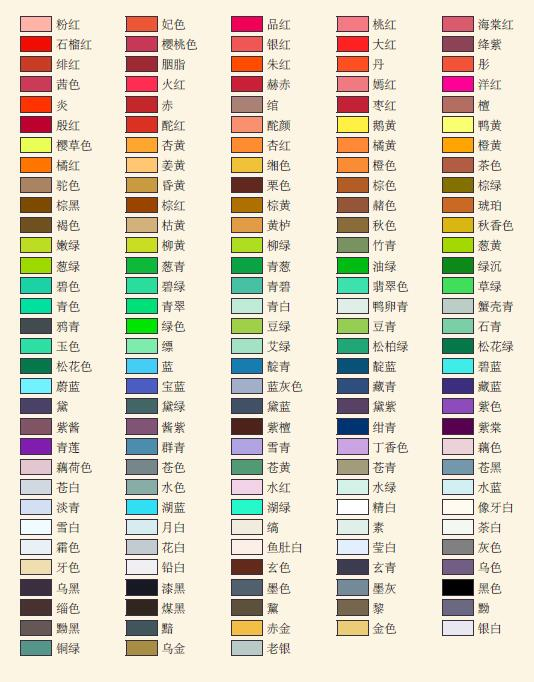
\includegraphics[width=0.65\textwidth]{pic11.jpg}

Texstudio菜单栏选项--设置Texstudio--语法高亮--正常--那一行(几个复选框后面,有三个调节颜色的色块,默认是没有的,自己手动调节第一个为字体颜色,第二个为编辑器背景颜色)豆沙绿RGB为199,237,204。

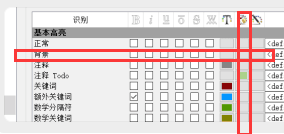
\includegraphics[width=0.65\textwidth]{pic12.png}

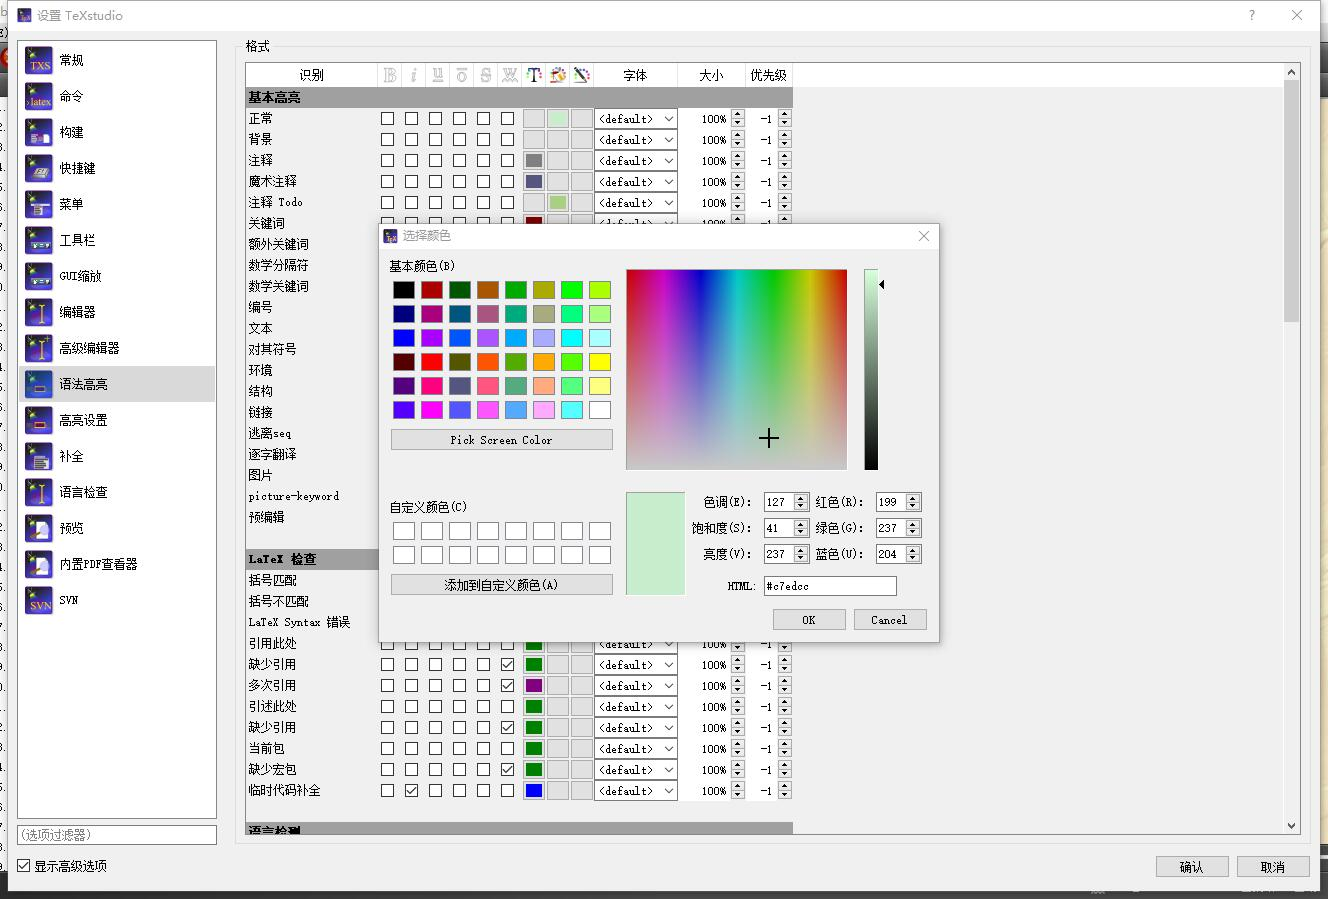
\includegraphics[width=0.65\textwidth]{pic13.jpg}

\begin{qst}\label{Q2018010804}
有一个问题不知道大家有没有遇到过,杂志社排版文章,下转XX页,上接XX页,这个有什么宏包可以实现么?\index{文档中上接下转}
\end{qst}
\ans 设置好锚点,交叉引用搞一下。

\begin{qst}\label{Q2018010805}
有没有制作奖状的模板?
\index{奖状模板}
\end{qst}
\ans 刚看到有人要做奖状?推一下这些可耐滴图案

 \href{https://github.com/liantze/pgfornament-han/}%
 {https://github.com/liantze/pgfornament-han/}  
 
 \href{http://tex.my/mail-merge-batch-generating-documents-with-datatool-package/}%
 {http://tex.my/mail-merge-batch-generating-documents-with-datatool\\-package/}

\begin{qst}\label{Q2018010806}
 集合之间不包含符号怎么输入?\index{不包含}
\end{qst}
\ans \verb| sprout  $\not\subset$|。

还可以看看手写符号识别\url{ http://detexify.kirelabs.org/classify.html}\index{手写符号识别}

\begin{qst}\label{Q2018010807}
全英文的文档怎么弄人民币符号?\index{RMB符号}
\end{qst}
\ans 导言区调用宏包\verb| \usepackage{textcomp}|, 正文中使用\verb|\textyen|得到\textyen.

还可以看看这个帖子\url{http://bbs.ctex.org/forum.php?mod=viewthread&tid=76024}

\end{document} 